\documentclass[a4paper,11pt]{report}
\usepackage{natbib}
\usepackage{subcaption}
\usepackage{cleveref}
\usepackage{packages/rapportutc}
\usepackage[nottoc, notlof, notlot]{tocbibind}
\usepackage{sidecap}
\usepackage{array}
\usepackage[linewidth=1pt]{mdframed}
\usepackage{float}


\usepackage{packages/Sweave} %package d'affichage des codes R
\usepackage{amsmath, amsthm, amssymb, graphics, setspace} %packages de mathématiques
\usepackage{calc,enumitem}  % Mise en forme l'environnement itemsize description etc.
%\usepackage{subfigure, wrapfig} % pour avoir plusieurs figures alignées  
\usepackage{color}
\usepackage{ae,aecompl}
\usepackage{pifont}
\usepackage{chemist} %formule chimique 
\usepackage{comment}
\usepackage{rotating}
\usepackage{hyperref}
\usepackage{listings}

\usepackage{setspace}

\onehalfspacing



%\usepackage{biblatex}

%%%%%%%%%%%%%%%%%%%%%%%%%%%%%%%%%%%%%%%%%%%%%%%%%%%%%%%%%%%%%%%%%%%%%%%%%%%% 

\title{TP 1 - Statistique descriptive, Analyse en composantes principales}
\author{LU Han - HAMONNAIS Raphaël}
\date{\today}

\uv{SY09}
\branche{Génie Informatique}
\filiere{Fouille de Données et Décisionnel}
%%%%%%%%%%%%%%%%%%%%%%%%%%%%%%%%%%%%%%%%%%%%%%%%%%%%%%%%%%%%%%%%%%%%%%%%%%%%

\begin{document}
\renewcommand{\labelitemi}{\large\textcolor{tatoebagreen}{\fg}}
\newgeometry{top=2.5cm,bottom=2cm,left=2cm,right=2cm}
\groovypdtitre
\restoregeometry % restaure la géométrie par défaut de latex

%%%%%%%%%%%%%%%%%%%%%%%%%%%%%%%%%%%%%%%%%%%%%%%%%%%%%%%%%%%%%%%%%%%%%%%%%%%% 

\tableofcontents

%%%%%%%%%%%%%%%%%%%%%%%%%%%%%%%%%%%%%%%%%%%%%%%%%%%%%%%%%%%%%%%%%%%%%%%%%%%%



\chapter{Statistique descriptive}

\section{Notes de SY02 au semestre de printemps 2016}

\subsection{Analyse descriptive}

\subsubsection{Description des données}


Le jeu de données contient des informations relatives aux 296 étudiants inscrits à l’UV SY02 au semestre de printemps 2016 ainsi que les résultats qu'ils ont obtenus. On a donc 296 mesures (individus de la population) représentés par onze variables~: 8 qualitatives et 3 quantitatives.\\
Liste des variables qualitatives~:
\begin{itemize}
	\item \textbf{nom} : nom de l'étudiant, au format texte (noms anonymisés, au format "\textit{Etu1, Etu2,~...}").
	\item \textbf{specialite} : spécialité de l'étudiant, $\in$ \{GB, GI, GM, GP, GSM, GSU, HuTech, ISS, TC\}.
	\item \textbf{niveau} : le numéro du semestre actuel de l'étudiant, $\in \{1,2,3,4,5,6\}$.
	\item \textbf{statut} : vaut $ \{UTC,Echange\} $ selon que c'est un étudiant de l'UTC ou bien un étudiant originaire d'une autre université effectuant une partie de ses études à l'UTC.
	\item \textbf{dernier.diplome.obtenu} : le dernier diplôme obtenu par l'étudiant, $\in$ \{\textsc{autre 1er cycle, autre 2e cycle, autre diplome superieur, bac, bts, cpge, deug, dut, etranger secondaire, etranger superieur, ingenieur, licence, na's}\}.
	\item \textbf{correcteur.median} et \textbf{correcteur.final} : le correcteur ayant corrigé la copie (nons anonymisés au format "\textit{Cor 1,~...}").
	\item \textbf{resultat} Le résultat de l'étudiant, de \textit{A} à \textit{F} ou \textit{ABS} s'il a été absent à l'un des deux examens (final ou médian). \textit{F} et \textit{Fx} signifient que l'étudiant n'a pas obtenu l'UV, les autres notes qu'il l'a obtenue.
\end{itemize}
Liste des variables quantitatives~:
\begin{itemize}
	\item \textbf{note.median} : la note obtenue au médian ($ \in [0;20] $).
	\item \textbf{note.final} : la note obtenue au final ($ \in [0;20] $).
	\item \textbf{note.totale} : la moyenne des deux notes, pondérée par l'importance de chaque note.
\end{itemize}


\subsubsection{Données manquantes}
On remarque qu'il manque certaines informations dans les données (R le spécifie avec le mot clé "\textit{NA's}" pour \textit{Not Available} en anglais)~:
\begin{itemize}
	\item Correcteur du médian et/ou du final~: élève absent au médian et/ou au final.
	\item Dernier diplôme obtenu~: donnée manquante pour les étudiants en échange.
	\item Note au médian et/ou au final~: donnée manquante pour les étudiants absents ou qui ont abandonné.
	\item Résultat~: donnée "manquante" pour R qui considère la valeur \textit{ABS} comme étant manquant car \textit{resultat} est une variable qualitative ordonnée et \textit{ABS} ne fait pas partie des différents niveau d'ordre. Représente donc des élèves absents qui n'ont pas obtenu l'UV.
\end{itemize}


\subsubsection{Intuitions statistiques~: liens supposés entre les variables}
De manière logique, on pourrait penser que les notes entre le médian et le final sont liées, un élève bon au médian étant plus à même de réussir le final et inversement. De même, la formation d'origine de l'étudiant devrait fortement influencer l'obtention de l'UV. Un étudiant venant de tronc commun (diplôme d'origine BAC) a logiquement plus de change de réussir qu'un élève venant de DUT. Le correcteur ne devrait logiquement pas influencer les notes, la notion d'équité entre les copies étant très importante.




\subsection{Etude des liens statistique entre les variables}

\subsubsection{Pré-requis}
On considère que les données ont été préalablement nettoyées en enlevant tous les étudiants absents, c'est à dire qui n'ont pas eu l'UV pour cause d'absence accidentelle ou d'abandon pur et simple.

\subsubsection{Procédure}

Nous utilisons le test d'indépendance du $\chi^2$ qui permet de vérifier l'indépendance de deux variables X et Y : 

\begin{itemize}
	\item Hypothèse nulle $H_{0}$~: les deux variables X et Y sont indépendantes.
	\item Hypothèse $H_{1}$~: les deux variables X et Y ne sont pas indépendantes.
	\item On rejette l'hypothèse nulle lorsque \textit{p-value} est inférieure ou égale à 0,05. La valeur \textit{p-value} représente la probabilité d'obtenir la même valeur (ou une valeur encore plus extrême) du test si l'hypothèse nulle était vraie.
	\item Toutes les cases du tableau de contingence doivent avoir une valeur supérieure ou égale à 5. Le tableau de contingence est un tableau à double entrée représentant les effectifs partiels des observations en fonction des variables X en ligne et Y en colonne.
\end{itemize}





\subsubsection{Lien statistique entre le résultat et le diplôme d'origine des étudiants}
La première étape fut de nettoyer les données en supprimant les 6 étudiants dont le statut vaut \textit{Echange} car leur diplôme d'origine n'est pas renseigné.\\
Nous avons ensuite créé le tableau de contingence, qui donne pour chaque valeur de la variable \textit{resultat} le nombre d'élèves ayant obtenu ce résultat en fonction de leur diplôme d'origine~: on obtient un effectif pour chaque couple \textit{diplôme d'origine}/\textit{résultat}.


\begin{figure}[H]
	\centering
	\captionsetup{justification=centering, margin=2cm}
	\begin{subfigure}[b]{0.5\linewidth}
		\centering
		\captionsetup{justification=centering, margin=1cm}
		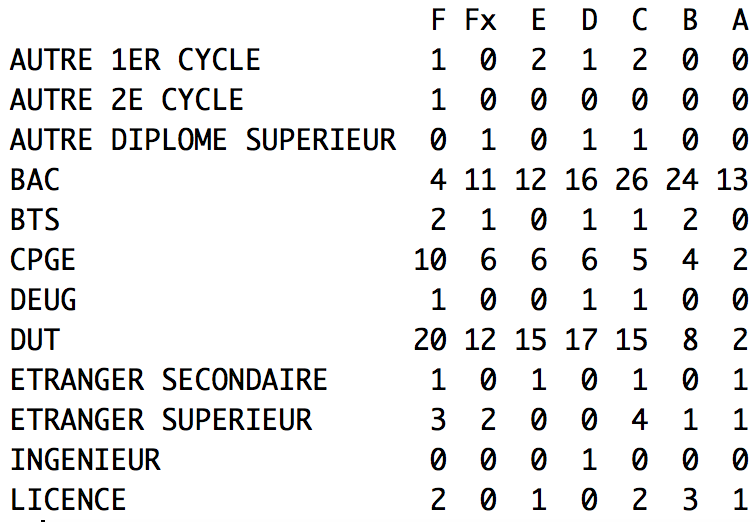
\includegraphics[width=0.65\linewidth]{img/1-1-2-Contingence-Result-Diplome-Origine}
		\caption{\scriptsize Tableau de contingence entre résultat et diplôme d'origine}
		\label{fig:tab_contingence_diplome_resultat}
	\end{subfigure}%
	\begin{subfigure}[b]{0.5\linewidth}
		\centering
		\captionsetup{justification=centering, margin=1cm}
		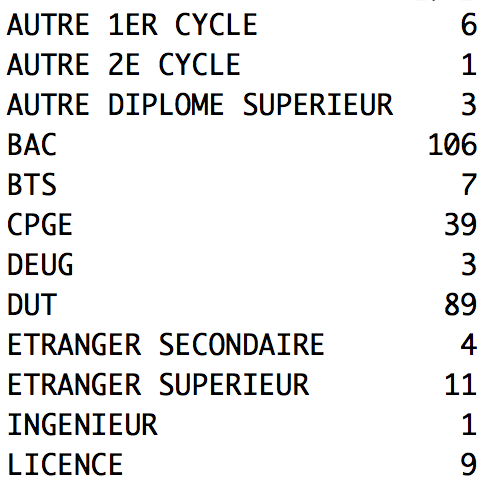
\includegraphics[width=0.5\linewidth]{img/1-1-2-Effectif-Diplome-Origine}
		\caption{\scriptsize Effectif total par diplôme}
		\label{fig:effectif_total_par_diplome}
	\end{subfigure}%
	\caption{
		\small Effectifs de la population par diplôme d'origine et tableau de contingence entre les variables \textit{résultat} et \textit{diplôme d'origine}.
	}
	\label{fig:tab_effectifs_et_contingence_resultats_diplome_origine}%
\end{figure}

On remarque immédiatement que les conditions du test ne sont pas respectées~: il a y une majorité des effectifs qui sont inférieurs à 5 dans le tableau de contingence  (\autoref{fig:tab_contingence_diplome_resultat}). Et c'est tout à fait normal si l'on regarde les effectifs d'étudiants (\autoref{fig:effectif_total_par_diplome}) en fonction de leur diplôme d'origine dans la population totale~: seuls les diplômes BAC (étudiant venant de tronc commun), DUT et CPGE sont convenablement représentés.
On peut tout de même effectuer le test du $\chi^2$ tout en sachant que les conditions ne sont pas respectées, afin de vérifier l'importance de ces conditions. On obtient alors une \textit{p-value} égale à $0.2572$. On conserve donc l'hypothèse $H_{0}$ d'indépendance des variables, tout en sachant que le résultat et probablement faux.



\paragraph{Correction des effectifs}
Afin de respecter les conditions du test de $\chi^2$, nous n'avons gardé que les lignes correspondant aux diplômes d'origines de type \textit{BAC}, \textit{DUT} et \textit{CPGE}. Il a aussi fallut regrouper les deux premières et deux dernières classes de \textit{résultat} en sommant les effectifs des élèves ayant obtenu \textit{F} ou \textit{Fx} et ceux ayant eu \textit{A} ou \textit{B}.\\
On obtient ainsi un nouveau tableau de contingence~:


\begin{figure}[H]
	\centering
	\captionsetup{justification=centering, margin=4cm}
	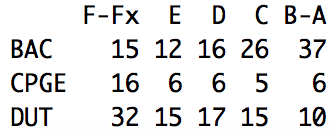
\includegraphics[width=0.3\linewidth]{img/1-1-2-Contingence-Result-Diplome-Corrigee}
	\caption{\scriptsize Tableau de contingence \textbf{corrigé} entre résultat et diplôme d'origine.}
	\label{fig:tab_effectifs_et_contingence_resultats_diplome_origine_corrigee}
\end{figure}
Les conditions du test sont alors réunies et on obtient une \textit{p-value} égale à $0.000288$. On rejette donc l'hypothèse $H_{0}$ d'indépendance avec confiance~: le diplôme d'origine d'un étudiant a un impact significatif sur son résultat final à l'UV de statistiques SY02.

Voici une représentation graphique de la fréquence des résultats en fonction du diplôme d'origine~:

\begin{figure}[H]
	\centering
	\captionsetup{justification=centering, margin=2cm}
	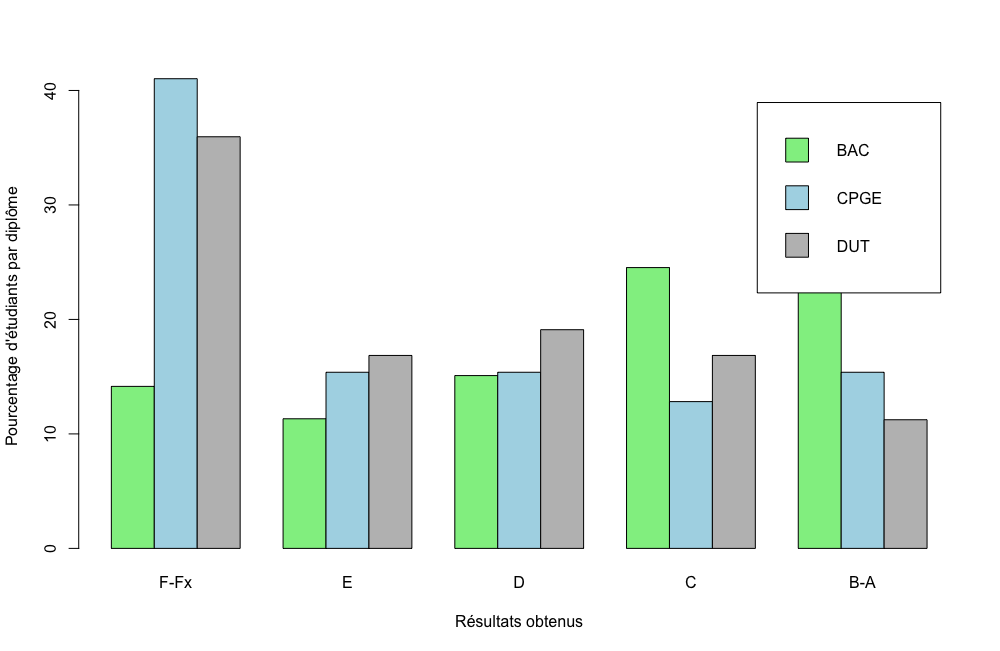
\includegraphics[width=.4\linewidth]{img/1-1-2-Ratio-resultat-diplome}
	\caption{\scriptsize Fréquence par diplôme d'origine et résultat}
	\label{fig:ratio_resultats_diplome}
\end{figure}


On remarque que 34\% des élèves ayant comme dernier diplôme le BAC ont obtenu \textit{A} ou \textit{B} tandis que seulement 14\% d'entre-eux n'ont pas réussi l'UV. On remarque aussi que la courbe est croissante~: plus le résultat est bon, plus la fréquence d'obtention augmente. C'est l'inverse pour les élèves provenant de DUT ou CPGE~: moins le résultat est bon, plus la fréquence d'élèves obtenant ce résultat augmente (environ 40\% des élèves en provenance d'un DUT ou de CPGE n'ont pas obtenu l'UV).


\subsubsection{Lien statistique entre le résultat et la spécialité des étudiants}

La spécialité des étudiants correspond à leur cursus actuel~: GB, GI, GM, GP, GSM, GSU, HuTech, ISS, ou TC. En s'intéressant à l'effectif de chaque classe (\autoref{fig:effectif_specialité}), on remarque de suite qu'il va falloir en considérer quelques unes seulement pour respecter les conditions du test.

\begin{figure}[H]
	\centering
	\captionsetup{justification=centering, margin=2cm}
	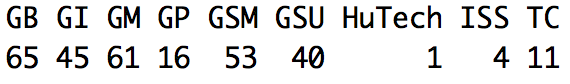
\includegraphics[width=.5\linewidth]{img/1-1-2-Effectf-specialite}
	\caption{\scriptsize Effectif par spécialité}
	\label{fig:effectif_specialité}
\end{figure}

Les classes telles que \textit{HuTech}, \textit{ISS}, \textit{TC} voire même \textit{GP} ne sont pas assez représentées pour être en mesure de respecter les conditions du tests d'indépendance du $\chi^2$.

Voici les deux tableaux de contingence obtenus, le premier sur toutes les données (\autoref{fig:tab_contingence_diplome_specialite_origine}), le second (\autoref{fig:tab_contingence_diplome_specialite_corrige}) en sélectionnant certaines classes de la variable \textit{spécialité} puis en regroupant les effectifs de certaines classes de la variable \textit{résultat}.

\begin{figure}[H]
	\centering
	\captionsetup{justification=centering, margin=2cm}
	\begin{subfigure}[b]{0.5\linewidth}
		\centering
		\captionsetup{justification=centering, margin=1cm}
		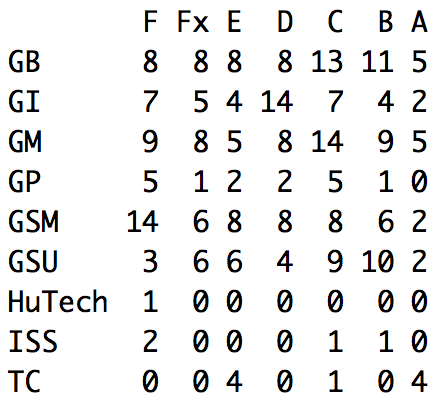
\includegraphics[width=0.5\linewidth]{img/1-1-2-Contingence-Result-Specialite-Origine}
		\caption{\scriptsize Tableau de contingence entre résultat et spécialité}
		\label{fig:tab_contingence_diplome_specialite_origine}
	\end{subfigure}%
	\begin{subfigure}[b]{0.5\linewidth}
		\centering
		\captionsetup{justification=centering, margin=1cm}
		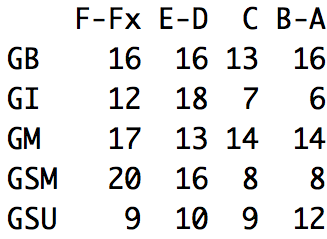
\includegraphics[width=0.5\linewidth]{img/1-1-2-Contingence-Result-Specialite-Corrige}
		\caption{\scriptsize Tableau de contingence \textbf{corrigé} entre résultat et spécialité}
		\label{fig:tab_contingence_diplome_specialite_corrige}
	\end{subfigure}%
	\caption{
		\small Tableaux de contingence entre résultats et spécialité.
	}
	\label{fig:tabs_contingence_resultats_specialite}%
\end{figure}

Les deux tests du $\chi^2$ effectués sur le tableau \ref{fig:tab_contingence_diplome_specialite_origine} et sur le tableau \ref{fig:tab_contingence_diplome_specialite_corrige} donnent respectivement les résultats suivants~:
\begin{itemize}
	\item Tableau de contingence d'origine
	\\ \textit{p-value} = 0.02087781.
	\\ On réfute (à tort) l'hypothèse $H_{0}$ d'indépendance des variables \textit{résultat} et \textit{spécialité}.
	
	\item Tableau de contingence corrigé
	\\ \textit{p-value} = 0.4673856.
	\\ On accepte l'hypothèse $H_{0}$ d'indépendance des variables \textit{résultat} et \textit{spécialité} avec confiance.
\end{itemize}

Conclusion~: la spécialité d'un étudiant n'a pas d'impact sur son résultat.


\subsubsection{Lien statistique entre le résultat et le niveau des étudiants}

Le niveau des étudiants correspond à leur semestre actuel de branche, de 1 à 6 (deux semestres par an sur un cursus de trois ans).

Voici les deux tableaux de contingences obtenus, le premier (\autoref{fig:tab_contingence_diplome_niveau_origine}) sans regroupement de classes et le second (\autoref{fig:tab_contingence_diplome_niveau_corrige}) en regroupant les classes \textit{F-Fx-E} et \textit{C-B} et en ne considérant pas les étudiants de niveau 3,5 et 6 (effectif trop peu important).

\begin{figure}[H]
	\centering
	\captionsetup{justification=centering, margin=2cm}
	\begin{subfigure}[b]{0.5\linewidth}
		\centering
		\captionsetup{justification=centering, margin=1cm}
		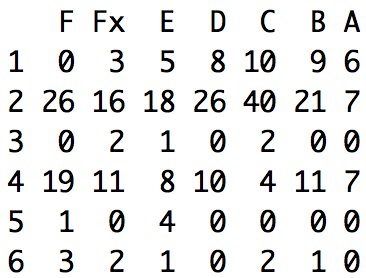
\includegraphics[width=0.5\linewidth]{img/1-1-2-Contingence-Result-Niveau-Origine}
		\caption{\scriptsize Tableau de contingence entre résultat et niveau}
		\label{fig:tab_contingence_diplome_niveau_origine}
	\end{subfigure}%
	\begin{subfigure}[b]{0.5\linewidth}
		\centering
		\captionsetup{justification=centering, margin=1cm}
		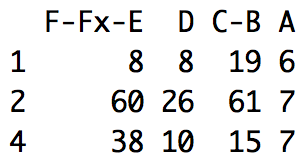
\includegraphics[width=0.5\linewidth]{img/1-1-2-Contingence-Result-Niveau-Corrige}
		\caption{\scriptsize Tableau de contingence \textbf{corrigé} entre résultat et niveau}
		\label{fig:tab_contingence_diplome_niveau_corrige}
	\end{subfigure}%
	\caption{
		\small Tableaux de contingence entre résultats et niveau.
	}
	\label{fig:tabs_contingence_resultats_niveau}%
\end{figure}


Les deux tests du $\chi^2$ effectués sur le tableau \ref{fig:tab_contingence_diplome_niveau_origine} et sur le tableau \ref{fig:tab_contingence_diplome_niveau_corrige} donnent respectivement les résultats suivants~:
\begin{itemize}
	\item Tableau de contingence d'origine
	\\ \textit{p-value} = 0.0003517831.
	\\ On réfute l'hypothèse $H_{0}$ d'indépendance des variables \textit{résultat} et \textit{niveau}.
	
	\item Tableau de contingence corrigé
	\\ \textit{p-value} = 0.003523739.
	\\ On réfute l'hypothèse $H_{0}$ d'indépendance des variables \textit{résultat} et \textit{niveau}.
\end{itemize}
Conclusion~: le niveau d'un étudiant impacte son résultat. On observe par exemple dans la figure \ref{fig:frequence_resultats_niveau} que plus le niveau de l'étudiant augmente, moins il a de chance d'obtenir l'UV. 42\% de \textit{F} ou \textit{Fx} pour les étudiants de niveau 4 contre 7\% seulement pour ceux de niveau 1. A l'opposé, ces derniers sont 80\% à obtenir l'UV avec un résultat entre \textit{D} et \textit{A} contre 45\% pour les étudiants de niveau 4. Les étudiants de niveau 2 se situent au milieu, avec 60\% pour un résultat compris entre \textit{D} et \textit{A} et 27\% de non obtention de l'UV.

\begin{figure}[H]
	\centering
	\captionsetup{justification=centering, margin=2cm}
	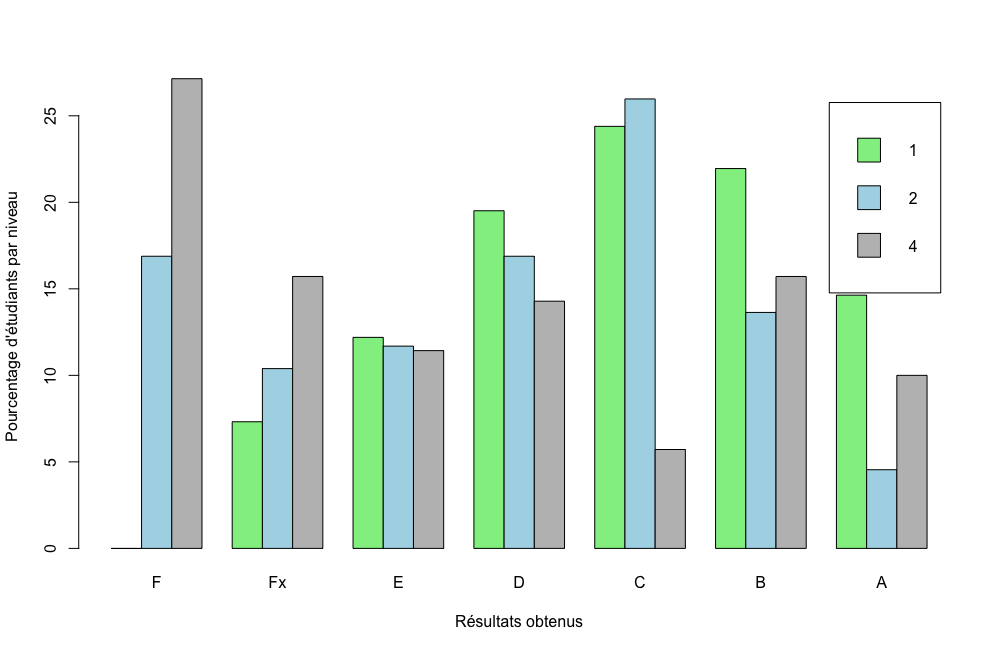
\includegraphics[width=.5\linewidth]{img/1-1-2-Ratio-resultat-niveau}
	\caption{\scriptsize Fréquence d'obtention d'un résultat en fonction du niveau de l'étudiant}
	\label{fig:frequence_resultats_niveau}
\end{figure}

\subsubsection{Lien statistique entre le résultat et les correcteurs}

Selon toute vraisemblance, le correcteur ne devrait pas influer sur le résultat d'un étudiant à l'UV. Nous allons tout de même nous en assurer. Le principe est le même que précédemment~: construire le tableau de contingence, regrouper des classes au besoin pour respecter les conditions du test du $\chi^2$ et effectuer ce test afin de déterminer si les variables sont indépendantes ou non.
\\
Voici le premier tableau de contingence obtenu entre les variable \textit{notes médian} et \textit{correcteur médian}~:

\begin{figure}[H]
	\centering
	\captionsetup{justification=centering, margin=2cm}
	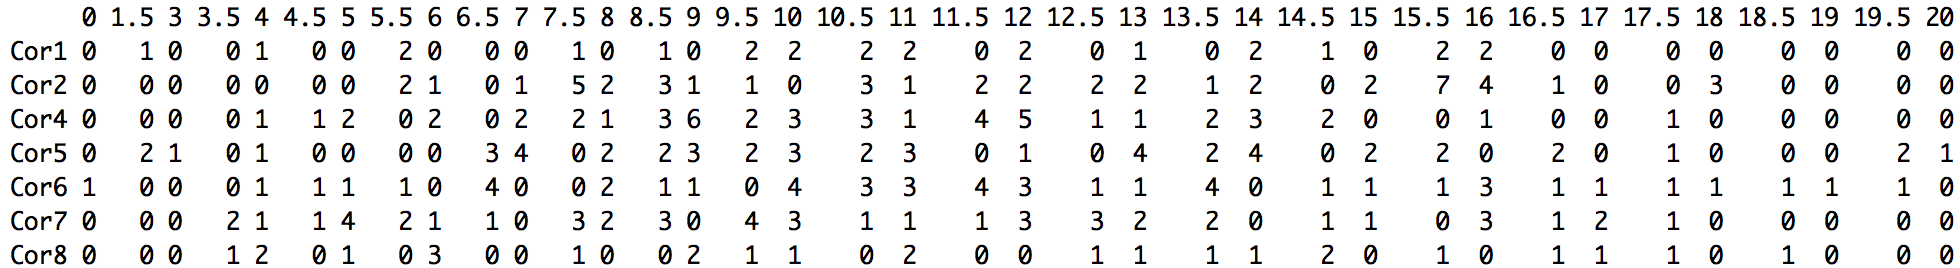
\includegraphics[width=.9\linewidth]{img/1-1-2-Contingence-Result-Correcteur-Median-Origine}
	\caption{\scriptsize Tableau de contingence entre les notes du médian et les correcteur}
	\label{fig:contingence_resultats_correcteur}
\end{figure}

Ce tableau est inutilisable pour le test d'indépendance du $\chi^2$. Il a donc fallut regrouper les observation en classes.\\
Voici le second tableau de contingence obtenu après regroupement~:
\begin{figure}[H]
	\centering
	\captionsetup{justification=centering, margin=4cm}
	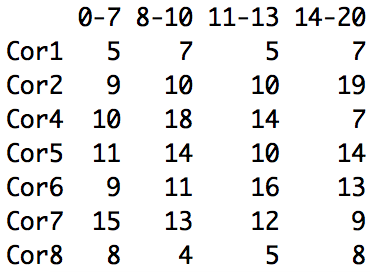
\includegraphics[width=.2\linewidth]{img/1-1-2-Contingence-Result-Correcteur-Median-Corrige}
	\caption{\scriptsize Tableau de contingence \textbf{après regroupement} entre les notes du médian et les correcteur}
	\label{fig:contingence_resultats_correcteur_corrige}
\end{figure}

Le test du $\chi^2$ effectué sur le second tableau de contingence donne une \textit{p-value} égale à 0.499. On conserve donc l'hypothèse $H{0}$ d'indépendance. Le même principe a été appliqué sur le couple de variable \textit{note final} et \textit{correcteur final} à la différence qu'il y a trois classes au lieu de 4 afin de respecter les conditions du test. La \textit{p-value} obtenue vaut 0.115. On conserve ici aussi l'hypothèse $H{0}$ d'indépendance.

Les notes obtenues au médian et au final étant fortement corrélées au résultat obtenu (\autoref{fig:boxplot_note_resultat}), on peut conclure en affirmant que les variables \textit{correcteur} et \textit{résultat} sont indépendantes.

\begin{figure}[H]
	\centering
	\captionsetup{justification=centering, margin=4cm}
	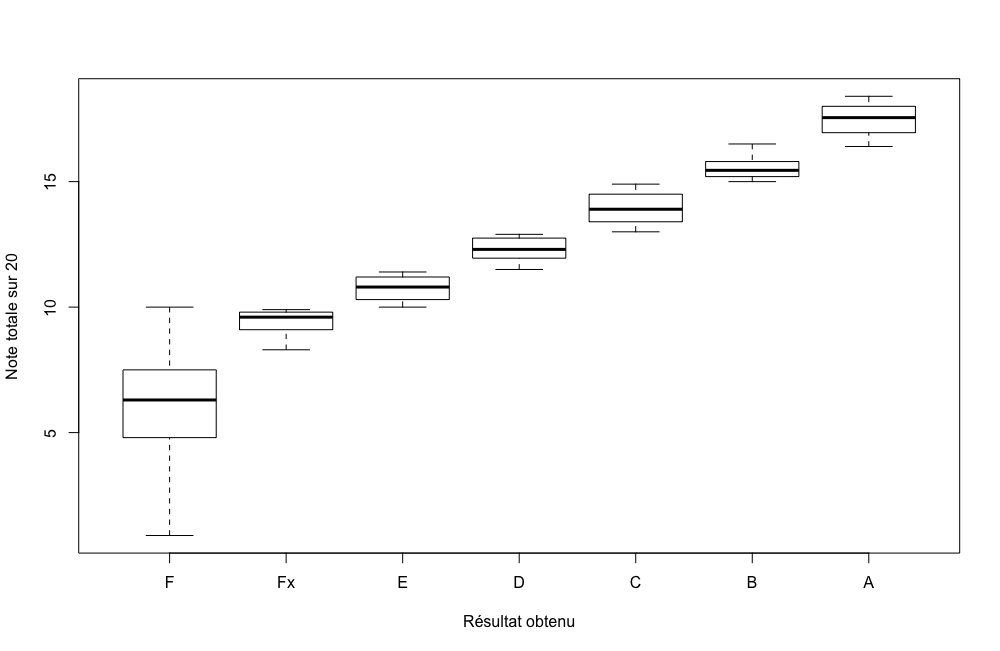
\includegraphics[width=.5\linewidth]{img/1-1-2-Boxplot-note-resultat}
	\caption{\scriptsize Distribution des résultats obtenus en fonction de la note finale}
	\label{fig:boxplot_note_resultat}
\end{figure}

\section{Données Crabs}

\subsection{Analyse descriptive}

\subsubsection{Description des données}

Le jeu de données présente 200 crabes classés en fonction de leur espèce et de leur sexe. Chaque individu est aussi décrit par 5 caractéristiques morphologiques quantitatives.
\\
Liste des variables qualitatives~:
\begin{itemize}
	\item \textbf{sex}~: le sexe du crabe, \textit{M} pour mâle, \textit{F} pour femelle.
	\item \textbf{sp}~: espèce à laquelle appartient un individu, \textit{O} pour \textit{Orange}, \textit{B} pour \textit{Bleu}.
\end{itemize}
Liste des variables quantitatives~:
\begin{itemize}
	\item \textbf{FL}~: taille de la frontale.
	\item \textbf{RW}~: largeur de la queue.
	\item \textbf{CL}~: longueur de la coquille.
	\item \textbf{CW}~: largeur de la coque.
	\item \textbf{BD}~: la profondeur du corps.
\end{itemize}
Il existe aussi une autre variable numérique, purement utilitaire, qui est l'index~:
\begin{itemize}
	\item \textbf{[1-50]}~: mâles d'espèce bleue.
	\item \textbf{[51-100]}~: femelles d'espèce bleue.
	\item \textbf{[101-150]}~: mâles d'espèce orange.
	\item \textbf{[151-200]}~: femelles d'espèce orange.
\end{itemize}


\subsubsection{Données morphologiques}

Les deux figures suivantes présentent les distributions des variables morphologiques en fonction de l'espèce (\autoref{fig:morphemetriques_en_fonction_espece}) et du sexe (\autoref{fig:morphemetriques_en_fonction_sexe}).\\


\begin{figure}[H]
	\centering
	\captionsetup{justification=centering, margin=2cm}
	\begin{subfigure}[b]{0.3\linewidth}
		\centering
		\captionsetup{justification=centering, margin=1cm}
		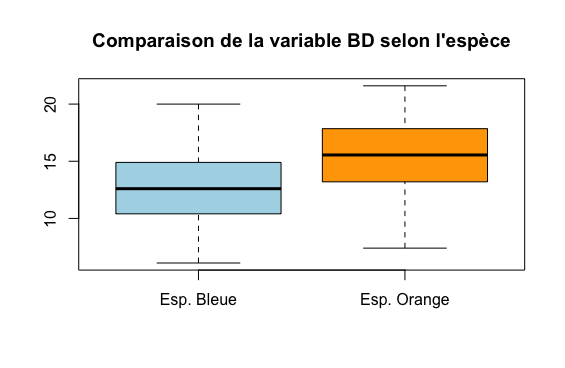
\includegraphics[width=1\linewidth]{img/1-2-1-espece-bd.png}
		\caption{\scriptsize Variable BD}
		\label{fig:1_2_1_espece_bd}
	\end{subfigure}%
	\begin{subfigure}[b]{0.3\linewidth}
		\centering
		\captionsetup{justification=centering, margin=1cm}
		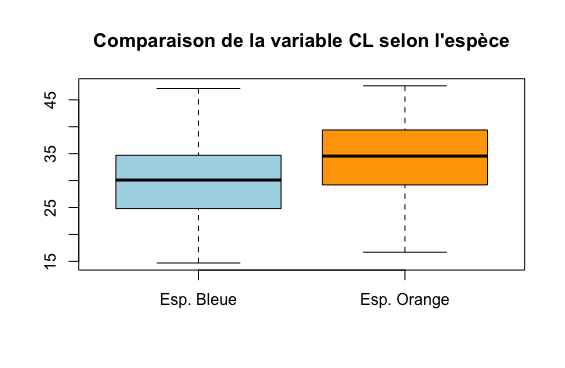
\includegraphics[width=1\linewidth]{img/1-2-1-espece-cl.png}
		\caption{\scriptsize Variable CL}
		\label{fig:1_2_1_espece_cl}
	\end{subfigure}%
	\begin{subfigure}[b]{0.3\linewidth}
		\centering
		\captionsetup{justification=centering, margin=1cm}
		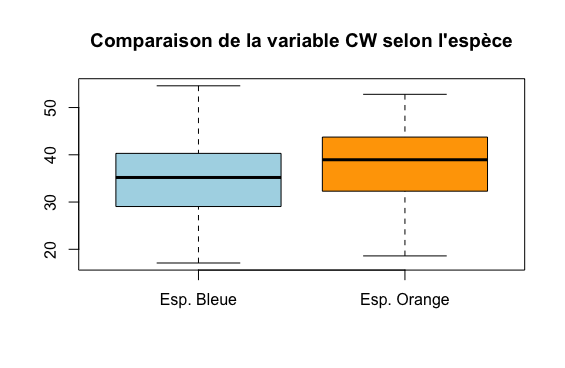
\includegraphics[width=1\linewidth]{img/1-2-1-espece-cw.png}
		\caption{\scriptsize Variable CW}
		\label{fig:1_2_1_espece_cw}
	\end{subfigure}%
	\\
	\begin{subfigure}[b]{0.3\linewidth}
		\centering
		\captionsetup{justification=centering, margin=1cm}
		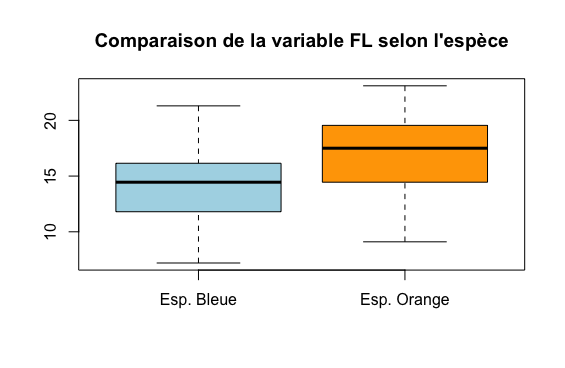
\includegraphics[width=1\linewidth]{img/1-2-1-espece-fl.png}
		\caption{\scriptsize Variable FL}
		\label{fig:1_2_1_espece_fl}
	\end{subfigure}%
	\begin{subfigure}[b]{0.3\linewidth}
		\centering
		\captionsetup{justification=centering, margin=1cm}
		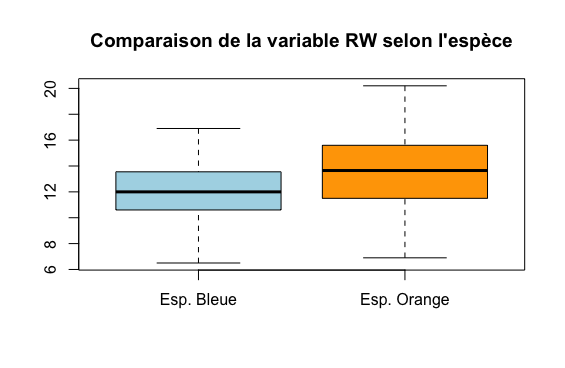
\includegraphics[width=1\linewidth]{img/1-2-1-espece-rw.png}
		\caption{\scriptsize Variable RW}
		\label{fig:1_2_1_espece_rw}
	\end{subfigure}%
	\caption{
		\small Distributions des variables morphométriques en fonction de l'espèce.
	}
	\label{fig:morphemetriques_en_fonction_espece}%
\end{figure}%

\begin{figure}[H]
	\centering
	\captionsetup{justification=centering, margin=2cm}
	\begin{subfigure}[b]{0.3\linewidth}
		\centering
		\captionsetup{justification=centering, margin=1cm}
		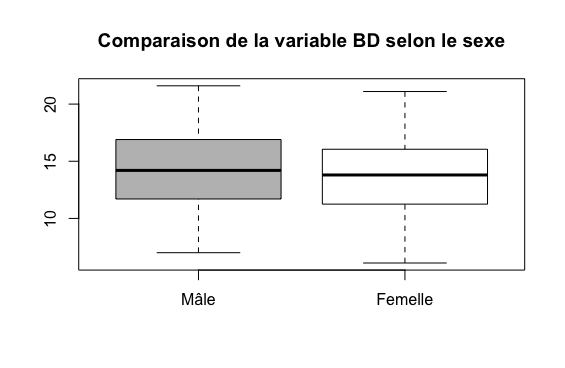
\includegraphics[width=1\linewidth]{img/1-2-1-sex-bd.png}
		\caption{\scriptsize Variable BD}
		\label{fig:1_2_1_sex_bd}
	\end{subfigure}%
	\begin{subfigure}[b]{0.3\linewidth}
		\centering
		\captionsetup{justification=centering, margin=1cm}
		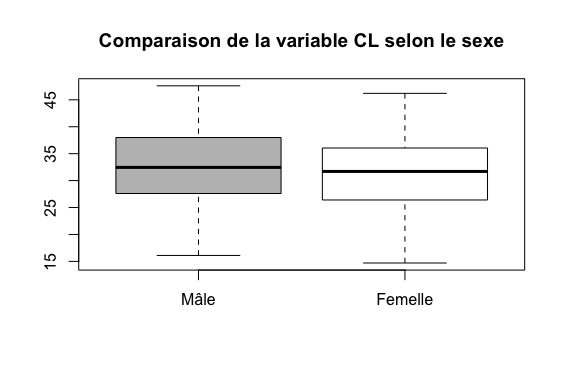
\includegraphics[width=1\linewidth]{img/1-2-1-sex-cl.png}
		\caption{\scriptsize Variable CL}
		\label{fig:1_2_1_sex_cl}
	\end{subfigure}%
	\begin{subfigure}[b]{0.3\linewidth}
		\centering
		\captionsetup{justification=centering, margin=1cm}
		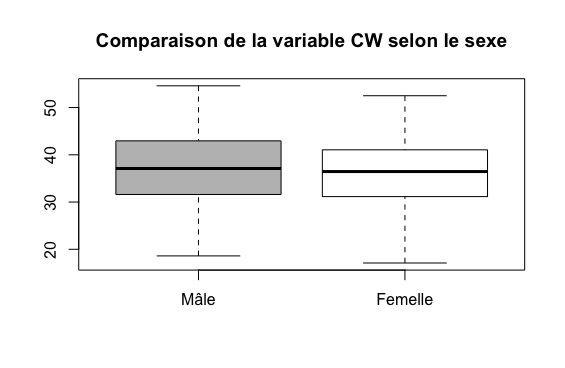
\includegraphics[width=1\linewidth]{img/1-2-1-sex-cw.png}
		\caption{\scriptsize Variable CW}
		\label{fig:1_2_1_sex_cw}
	\end{subfigure}%
	\\
	\begin{subfigure}[b]{0.3\linewidth}
		\centering
		\captionsetup{justification=centering, margin=1cm}
		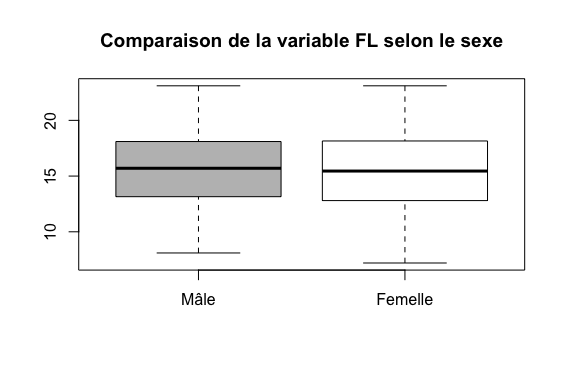
\includegraphics[width=1\linewidth]{img/1-2-1-sex-fl.png}
		\caption{\scriptsize Variable FL}
		\label{fig:1_2_1_sex_fl}
	\end{subfigure}%
	\begin{subfigure}[b]{0.3\linewidth}
		\centering
		\captionsetup{justification=centering, margin=1cm}
		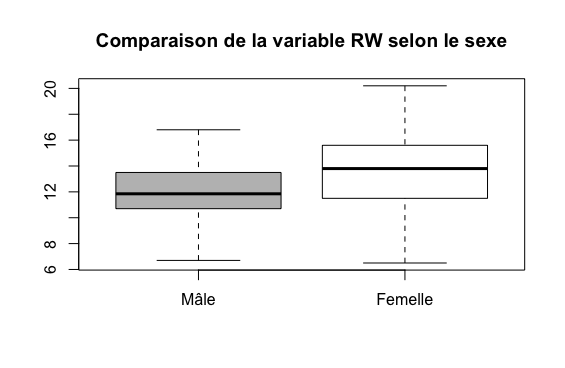
\includegraphics[width=1\linewidth]{img/1-2-1-sex-rw.png}
		\caption{\scriptsize Variable RW}
		\label{fig:1_2_1_sex_rw}
	\end{subfigure}%
	\caption{
		\small Distributions des variables morphométriques en fonction du sexe.
	}
	\label{fig:morphemetriques_en_fonction_sexe}%
\end{figure}

Graphiquement, il semble difficile de séparer les individus en fonction de leur sexe ou de leur espèce. Comparer les populations de même sexe mais d'espèce différente, de même espèce mais de sexe différent ou encore de sexe et espèce différents donne des résultats similaires. Aucune de ces variables, prise individuellement, ne nous permet d'identifier le sexe ou l'espèce d'un individu.

\subsection{Etude de la corrélation entre les variables morphologiques}

La corrélation entre les cinq variables est très forte, comme le montre le tableau de corrélation suivant~:
\newpage
\begin{table}[h]
	\centering
	\captionsetup{justification=centering, margin=2cm}
	\caption{Corrélations entre les variables quantitatives de la population de crabes.}
	\begin{tabular}{rrrrrr}
		\hline
		& FL & RW & CL & CW & BD \\ 
		\hline
		FL & 1.00 & 0.91 & 0.98 & 0.96 & 0.99 \\ 
		RW & 0.91 & 1.00 & 0.89 & 0.90 & 0.89 \\ 
		CL & 0.98 & 0.89 & 1.00 & 1.00 & 0.98 \\ 
		CW & 0.96 & 0.90 & 1.00 & 1.00 & 0.97 \\ 
		BD & 0.99 & 0.89 & 0.98 & 0.97 & 1.00 \\ 
		\hline
	\end{tabular}
\end{table}


La raison de cette forte corrélation est que les variables représentent des mesures morphométriques, c'est à dire des distances relevées sur les corps des crabes. Plus un crabe est grand, plus ces mesures vont grandir, et inversement.
Pour s'affranchir de ce phénomène, on pourra pratiquer une analyse en composantes principales sur les données. Les nouvelles variables identifiées auront alors une très faible corrélation entre elles. Il sera alors peut-être possible de différencier le sexe et l'espèce des individus en fonction de leur mesures morphométriques analysées en fonction des nouveaux axes trouvées lors de l'ACP (voir \autoref{sec:2_3_ACP_Crabs}).


\section{Données Pima}




\chapter{Analyse en composantes principales}


\section{Exercice théorique}


\section{Utilisation des outils R}


\section{Données Crabs}
\label{sec:2_3_ACP_Crabs}

\section{Données Pima}
\label{sec:2_4_ACP_Pima}




\end{document}